\chapter{Underground Infrastructure}
\label{ch:fscf-und-infra}

The requirements for underground infrastructure for the LBNF Project will be satisfied by a combination of existing infrastructure, improvements to this infrastructure, and development of new infrastructure to suit specific needs. The Project is aware that %must consider the 
other tenants underground at SURF, %for which 
including both the existing Davis Campus experiments and the Ross Campus experiments, 
will also require this infrastructure. % is required, 
The Ross campus experiments in particular are in relatively close proximity ($\sim$150~m) to LBNF.
%\fixme{what does it mean `consider'? Limitations will be imposed on LBNF due to the needs of the other tenants?  please clarify}

The infrastructure must support (1) the FSCF %LBNF Conventional Facilities (CF) 
construction activities, (2) installation of the Cryogenics Infrastructure and the experiment, and (3) operation of all the %both CF 
the equipment and the experiment. 
After analysis of these activities, the most stringent requirements that they impose 
%These three scenarios were analyzed and the most demanding requirements chosen from each situation 
were used to define the requirements for design.

Among the requirements is the need to reduce the risk of existing infrastructure failure to be able to adequately support LBNF construction
 activities. This work will be completed as Site Preparation: Ross Shaft rehabilitation,  maintenance and repair focused on the Yates Shaft, and ground-support activities at the 4850L between the Yates and Ross Shafts. Additional discussion of this work is included in Section 3.5 \fixme{ref}.

%Some of the SURF infrastructure that requires upgrading for LBNF will be rehabilitated prior to the beginning of LBNF construction funding. This includes Ross Shaft rehabilitation, Yates Shaft focused maintenance and repair \fixme{Elaine put this in parens, why?}, and ground support activities at the 4850L between the Yates and Ross Shafts. Additional discussion of this work is included in section 3.5 \fixme{ref}.

The preliminary design for LBNF underground infrastructure has been produced collaboratively, %several entities. 
the primary designer  %referenced in this document 
being Arup, USA. %Arup's 
The scope of this design %includes utility provisions and fire protection-life safety (FLS) strategy, 
covers infrastructure from the surface down through the shafts and drifts, to the excavations for the detector modules. Arup's design %incorporates the experiment's utility requirements \fixme{why call this out specifically?}  %provided by DUNE and and 
was produced in coordination with LBNF, SURF and the excavation and surface design teams. 

The utility infrastructure includes fire/life safety systems and strategies, permanent ventilation pathways, %guidance, 
HVAC, power, plumbing systems, communications infrastructure, lighting and controls. The design is fully documented in Arup's LBNF 100\% Preliminary Design Report\cite{arup:fscf100pdr} and in the preliminary design drawings. This chapter includes a summary of %the work done by Arup and utilizes information from 
that report.

Shaft rehabilitation and waste-rock handling design were previously provided for the DUSEL PDR in 2011 and LBNF will follow this design. This chapter uses excerpts from the DUSEL Preliminary Design Report, Chapter 5.4 [10] \fixme{xref and citation}. The research supporting this work took place in whole or in part at SURF, which was then called the Sanford Underground Laboratory at Homestake in Lead, South Dakota. Funding for this work was provided by the National Science Foundation through Cooperative Agreements PHY-0717003 and PHY-0940801. The assistance of the Sanford Underground Laboratory at Homestake and its personnel in providing physical access and general logistical and technical support is acknowledged.

%%%%%%%%%%%%%%%%%%%%%%%%%%%%%%%%%%%%%%%%%%%%%%%%%%%%%%%%%%%%%%%%%%%
\section{Fire/Life Safety Systems}
\label{sec:fscf-und-fire}

Life safety is a significant design criterion for underground facilities, focusing on events that could impact the ability to safely %escape
evacuate personnel, or if evacuation is not immediately possible, isolate personnel from potentially dangerous situations %events 
underground. Design for fire events includes both preventing the spread of fire and removing smoke and/or cryogenic gases through the ventilation system. The evaluation and establishment of requirements for cryogenic gas removal is performed by the Cryogenics Infrastructure project team and provided to FSCF.

Arup identified the life safety requirements and developed the design, utilizing applicable codes and standards, including \textit{NFPA 520: Standard on Subterranean Spaces}, which requires adequate egress in the event of an emergency. Facility fire detection and suppression systems, as well as personnel occupancy requirements are defined in accordance with \textit{NFPA 101: Life Safety Code}. The design was reviewed by Aon Risk Solutions and the recommendations documented in \textit{Fire Protection/Life Safety Assessment for the Conceptual Design of the Far Site of the Long Baseline Neutrino Experiment} \fixme{ref} [16]. Due to the unique nature of the experiment and its location, a number of potential variances will require approval from the authority having jurisdiction (AHJ). Significant examples include use of elevators for egress and use of drifts as air ducts. The AHJ for Lead, SD is familiar with the facility and the project, and is expected to provide reasonable and timely feedback for proposed variances.  

Based on data provided by SURF, the maximum occupant load of the 4850L will be limited to %controlled at 
144 following completion of the Ross Shaft Rehabilitation. This limit is based on both the ability of the shafts to provide egress within one hour and the capacity of the existing refuge chamber.  This chamber can support the anticipated 42 Underground Operations staff, 50 science staff for LBNF (during installation), and 20 science staff associated with the existing experiments. A logistics study\cite{lbnf-logistics} completed by Arup that evaluated the occupancy load during CF construction % as well, 
confirms the adequacy of this number.

To limit the horizontal and vertical spread of any fire or smoke, egress routes will be separated from adjacent spaces via  compartmentalization. This will also help limit the spread of %other materials such as 
any cryogenic gas leaks, or other leaks and spills. %This results in design criteria of 
%The resulting requirement is 
A minimum four-hour fire separation is required between the LBNF caverns and adjacent drifts, and a minimum two-hour fire separation for all rooms that connect directly to the egress drift at 4850L, as well as the shafts. %, will have 2-hour minimum fire separation.
Fire and life safety systems designed to meet these requirements % design criteria described above 
are described in the following sections.


%%%%%%%%%%%%%%%%%%%%%%%%%%%%%%%%%%%%%%%%%%%%%%%%%%%%%%%%%%%%%%%%%%%  to here 
\section{Shafts and Hoists}
\label{sec:fscf-und-shafts}

The Ross and Yates Shafts provide the only access/egress between the surface and the underground levels, and are therefore critical to the function of the facility. Both shafts provide service down to the 4850L, though not every intermediate level is serviced from both shafts. The shafts also provide a path for all utilities between the surface and the underground. 

The Ross and Yates Shafts were both installed in the 1930s and have operated since installation. These shafts, along with their furnishings, hoists and cages, were well maintained during mining operations, but experienced some deterioration in the years after the mine closed. %, as described in this section. 
A complete assessment of the Ross and Yates Shafts was conducted for the DUSEL Project in 2011, and is documented in the Arup Preliminary Infrastructure Assessment Report (DUSEL PDR Appendix 5.M [10]).\fixme{reference}



%%%%%%%%%%%%%%%%%%%%%%%%%%%%%%%%%
\subsection{Ross Shaft}
\label{sec:fscf-und-shafts-ross}

The Ross Shaft will be used for facility construction, including waste rock removal, routine facility maintenance, and as an egress path for the finished underground campuses. It will also be used for primary access to the DUNE experiment. Excavation for LBNF cannot begin until the Ross Shaft is rehabilitated by  SURF.

The Ross Shaft is rectangular in shape --- 14 ft 0 in (4.27 m) by 19 ft 3 in (5.87 m), measured to the outside of the set steel. The shaft collar is at elevation 5,354.88 ft (1,632.17 m) and the 5000L is the bottom level at elevation 277.70 ft (84.64 m) above sea level. 
 Service is provided to 29 levels and five skip loading pockets. The shaft is divided into seven compartments: cage, counterweight, north skip, south skip, pipe, utility, and ladder way. Figure~\ref{fig:ross-shaft-set} shows the shaft cross sectional layout. %\fixme{on figure,  `mT' is metric ton}


\begin{cdrfigure}[Ross Shaft, typical shaft set]{ross-shaft-set}{Ross Shaft, typical shaft set (SRK, Courtesy SURF)}
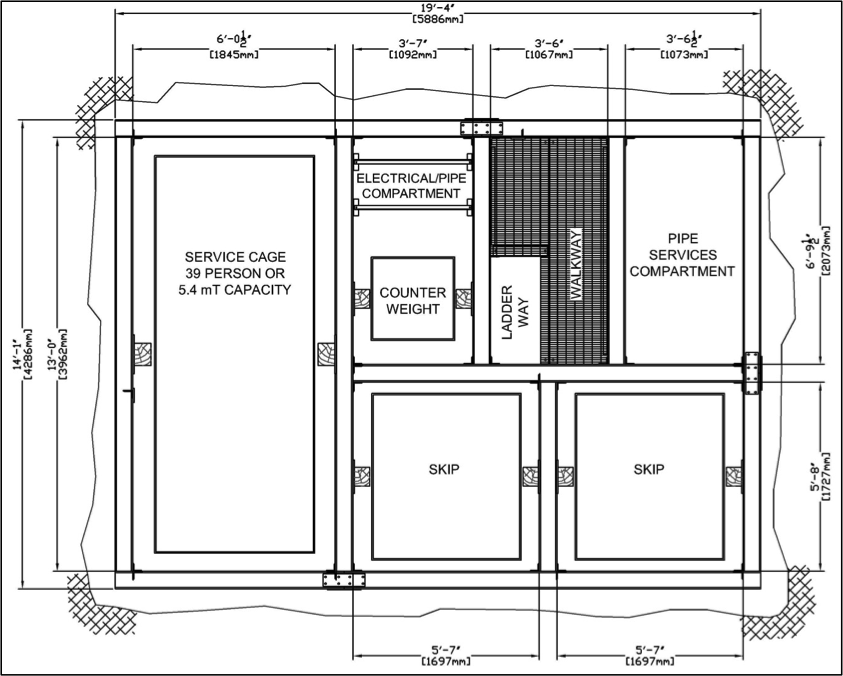
\includegraphics[width=0.8\textwidth]{ross-shaft-set}
\end{cdrfigure}

The Ross Shaft was in operation until the Homestake Gold Mine closed in 2003, and was put back in operation when the Sanford Laboratory reopened
 the site in 200x \fixme{year} without major repairs.  Deterioration through corrosion and wear on the shaft steel, including studdles (vertical steel members placed between steel sets), sets, and bearing beams, prompted a full \textit{strip and re-equip} project presently being performed by  SURF. %The shaft layout will not be significantly modified from the existing configuration. 
The set spacing is being increased from 6 ft to 18 ft, but the general configuration of the shaft will remain the same to allow it to remain in service for emergency egress during rehabilitation. \fixme{because that requires less work? what's connection between config and allowing egress?} 
The shaft was installed with limited ground support in the surrounding walls, electing to utilize lacing to prevent spalled rock from reaching the personnel conveyances. %\fixme{I have no idea what prev sentence means, i.e. how these things relate to each other. Wait, is ground support something in the rock walls around the shaft? then lacing is some kind of non-solid wall around the cage that carries people?} 
The new design replaces this system with a pattern bolting system to control rock movement. 
%The requirements for this shaft are safety, performance, and code driven and defined by the existing configuration. 
The requirements for this shaft are constrained by the existing configuration; they are driven by a focus on safety, performance, and codes.
%
Shaft rehabilitation through calendar year 2016 is being executed by SURF with non-LBNF Project funds. The rehabilitation is just over 60\% complete as of this report and completion is planned for 2017. Beginning in January 2017, the funding for the balance of the rehabilitation project will come from the LBNF Project as part of site preparation (Chapter~\ref{ch:fscf-site-prep}).  This will also include rehabilitation of the skip loading pocket for waste rock handling, and replacement of skips, cage, and ropes.

The production and service hoists at the Ross Shaft are located on the surface in a dedicated hoistroom west of the shaft. The service hoist operates the service cage and the production hoist operates the production skips. The DUSEL PDR \fixme{ref} describes the condition assessment of the electrical and mechanical hoisting systems which are described in detail in the Arup Preliminary Infrastructure Assessment Report (DUSEL PDR Appendix 5.M [10]\fixme{ref} ). These electrical and mechanical systems will have standard maintenance performed on them to restore them to like-new condition, but will not be modified from the existing design. %The Ross Headframe steel requires some strengthening and modifications to meet code requirements. 
All of this work is captured in the LBNF scope as part of site preparation (Chapter~\ref{ch:fscf-site-prep}).

%%%%%%%%%%%%%%%%%%%%%%%%%%%%%%%%%
\subsection{Yates Shaft}
\label{sec:fscf-und-shafts-yates}

The Yates Shaft is rectangular in shape -- 15 ft 0 in (4.572 m) by 27 ft 8 in (8.433 m) -- measured to the outside of the set timbers. There are two cage compartments and two skip compartments as shown in Figure~\ref{fig:yates-shaft}. In addition to the cage and skip compartments, two other compartments accommodate shaft services. The shaft collar is at 5,310.00 ft (1,618.49 m) elevation and the 4850L is the bottom level at elevation 376.46 ft (114.75 m) above sea level. Service is provided to 18 levels plus four skip-loading pockets. Sets are made up of various length and size timbers located so as to maintain compartment spaces. 
% \fixme{what's a `set' and is `size' really thickness? Are the timbers the structural pieces that are placed between compartments?}
 The Yates Shaft is timbered except for a fully concrete-lined portion from the collar to the 300L. Recent repairs include full set replacement from the concrete portion to the 800L and additional set repair below this level where deemed critical.

The Yates Service Hoist and Production Hoist are planned to be used as they are, with maintenance performed to bring them into like-new condition as part of site preparation (Chapter~\ref{ch:fscf-site-prep}). Further details regarding the condition of the Yates Hoists' electrical and mechanical condition can be found in Section 2.2 of the Arup Preliminary Site Assessment Report (DUSEL PDR Appendix 5.M) \fixme{citation}.

\begin{cdrfigure}[Existing Yates Shaft layout ]{yates-shaft}{Existing Yates Shaft layout (Adapted from SRK, Courtesy SURF)}
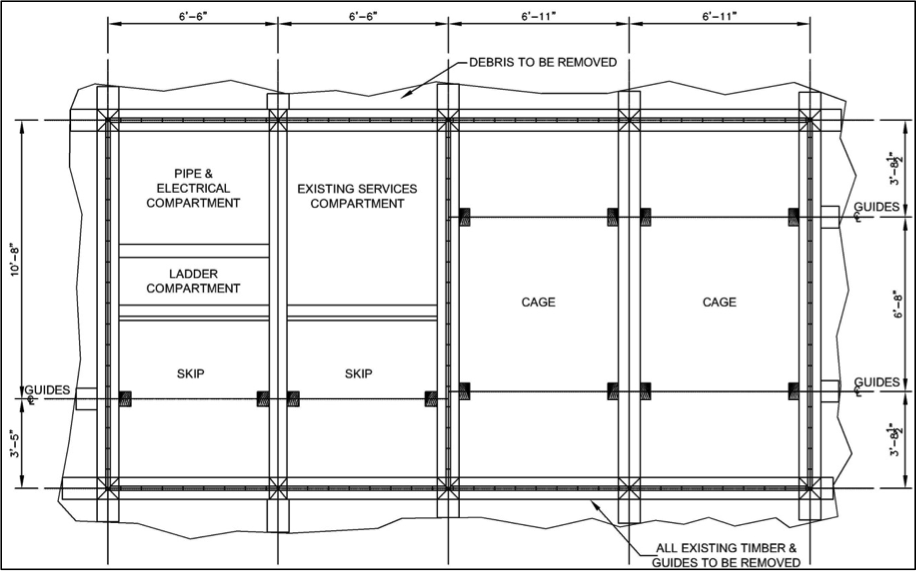
\includegraphics[width=0.8\textwidth]{yates-shaft}
\end{cdrfigure}



%%%%%%%%%%%%%%%%%%%%%%%%%%%%%%%%%%%%%%%%%%%%%%%%%%%%%%%%%%%%%%%%%%%
\section{Ventilation}
\label{sec:fscf-und-vent}

The ventilation system for LBNF/DUNE will utilize the existing mine ventilation system for most of the distance to the surface, with modifications made near the LBNF caverns to improve capacity. Fresh air for the LBNF caverns and the utility drifts will be provided by pulling air directly from the existing drifts, which is supplied from the Yates and Ross Shafts. 
%
Air will be exhausted from the LBNF cavities and utility drifts through a spray chamber, the primary function of which is rejecting heat from the LBNF chilled water system (see Section~\ref{sec:fscf-und-ch-h2o}). In this chamber 
the exhaust and heat are directed into a new borehole that connects to the 3500L at a point near the Oro Hondo shaft. The mixture is routed to the shaft, and pulled directly up by the fan at the surface.

The design calls for a ventilation rate for heat extraction of 230,000 cfm 
of which  27,500 cfm passes through each detector cavern and 21,500 through the Central Utility Cavern; the balance of the air required for heat rejection will come directly from the shafts through connections to existing drifts. The environmental design criteria for LBNF underground spaces are shown in Table~\ref{tab:env-design-crit}.

\begin{cdrtable}[Environmental design criteria (Arup)]{lllccl}{env-design-crit}{Environmental design criteria (Arup)}
Room & Internal         & Humidity & Min. Vent. Rate/   & Occupancy   \\
         & Temperature & Range     & Fresh Air Changes  & (during assembly)  \\  \toprowrule 

LBNF Cavities & $40 - 82\,^{\circ}\mathrm{F}$ & $15 - 85\%$ & 1& 20(50)~\tablefootnote{During operations, occupancy of the LBNF cavities is 20. Temperature, humidity and filtration requirements in localized areas of these spaces may differ, dependent on requirements. This will be provided by the experiment installation design team. The internal conditions stated above will be used to inform the design of plant and services for each space unless specific requirements that differ from this are provided by LBNF/SURF or the lab experiment design teams.} \\ 
                      & ($10 - 28\,^{\circ}\mathrm{C}$) & & & \\ \colhline
Access Drifts & Min $50\,^{\circ}\mathrm{F}$ & Uncontrolled & & Transient\\ 
                     & ($10\,^{\circ}\mathrm{C}$) &  & & space \\ \colhline
Utility spaces / & $50 - 95\,^{\circ}\mathrm{F}$ & Uncontrolled & 1& \\ 
Electrical rooms & ($10 - 35\,^{\circ}\mathrm{C}$) &  & & \\ \colhline
Storage Rooms & $59 - 104\,^{\circ}\mathrm{F}$ & Uncontrolled&Min 15 & Room-\\
                        & ($15 - 40\,^{\circ}\mathrm{C}$) & & cfm/person & dependent\\ 
\end{cdrtable}


Per historical data, outdoor temperatures can drop below $-20\,^{\circ}\mathrm{F}$; therefore, the intake air requires heating to prevent ice build-up in the shafts which could potentially disrupt hoisting operations and damage shaft support members, cables and piping. The existing shaft heaters are expected to be adequate for normal operation, but temporary supplemental heating may be necessary during excavation due to higher demands.  A study will be performed during final design to determine if waste heat from the cryogenics systems surface compressors can be used for energy savings to heat the intake air. %\fixme{I guess cryo systems will be operating for excav of chambers 2 (partial), 3 and 4?}

%%%%%%%%%%%%%%%%%%%%%%%%%%%%%%%%%%%%%%%%%%%%%%%%%%%%%%%%%%%%%%%%%%%
\section{Electrical}
\label{sec:fscf-und-elec}


%%%%%%%%%%%%%%%%%%%%%%%%%%%%%%%%%%
\subsection{Normal Power}
\label{sec:fscf-und-norm-pwr}

The estimated electrical loads for both the far detector and the underground infrastructure serving the detector spaces are included in the facility load determination and design; the loads are listed in Table~\ref{tab:undergr-elec-loads}. 

Power for the far detector will originate from the Ross substation and be routed down the Ross Shaft to the 4850L. One set of 15-kV mining cables will be installed down the Ross Shaft to the 4850L. These will be cable-rated for mine use, highly flame retardant, have low smoke toxicity, high tensile strength and be self-supporting. At the 4850L, the 15-kV mining cables will terminate in a 15-kV switchgear located in a new Ross underground substation. This will be provided early in the construction process to allow it to be used for construction.


\begin{cdrtable}[Underground Electrical Loads]{lr}{undergr-elec-loads}{Underground Electrical Loads}
Underground Electrical Load by Area & kW  \\ \toprowrule
%
Cryostat 1\&2 Detector Electronics & 450 \\ 
Cryostat 1\&2 Argon Pumps & 98 \\ 
Cryostat 1\&2 CF & 350 \\  \colhline
Total Cryostat 1\&2 & 898\\ \colhline  \colhline
%
Cryostat 3\&4 Detector Electronics & 450 \\ 
Cryostat 3\&4 Argon Pumps & 98 \\ 
Cryostat 3\&4 CF & 342 \\ \colhline
Total Cryostat 3\&4& 890\\ \colhline \colhline
%
Central Utility Cavern - Detector Cryogenics & 956 \\ 
Central Utility Cavern - DAQ & 36 \\ 
Central Utility Cavern - CF & 753 \\ \colhline
Total Central Utility Cavern& 1745\\ \colhline \colhline
%
Spray Chamber & 165 \\ 
Maintenance/Assembly Shops (2) & 84 \\ 
Drifts & 152 \\ \colhline
Total (other spaces) & 401\\ \colhline \colhline
%
Total non-CF & 2088 \\ 
Total CF & 1846 \\  \colhline
\textbf{Total} & \textbf{3934} \\  \colhline
Aggregate Demand Factor & 0.736 \\ \colhline
\textbf{Total} $\times$ \textbf{Aggregate Demand Factor}  & \textbf{2894 }\\ 
\end{cdrtable}

\begin{cdrtable}[Surface Electrical Loads]{lr}{surface-elec-loads}{Surface Electrical Loads}
Surface Electrical Load & kW \\ \toprowrule
Cryogen Building & 5000 \\
Control Room & 250 \\ 
Emergency/Standby Generator & 50 \\  \colhline
\textbf{Total Surface Load} & \textbf{5300}\\ 
\end{cdrtable}


%%%%%%%%%%%%%%%%%%%%%%%%%%%%%%%%%%
\subsection{Standby and Emergency Power}
\label{sec:fscf-und-emerg-pwr}

Standby power is necessary for emergency %occupant 
evacuation of personnel %LAr experiment require standby power 
and circulation of cryogens (to avoid rapid boil-off and loss of argon) when surface power is inoperable.

A 300-kW emergency/standby diesel generator will be provided in the Central Utility Cavern with % to serve standby and emergency loads. 
48 hours worth of diesel fuel to operate it. This duration aligns with the stored LN for controlling argon boil off; these figures satisfy requirements derived from historical power outages at the facility.  Note that the facility is fed by the local utility provider in a loop infrastructure, and therefore power to the site has historically been very reliable -- on the order of a few hours down per year.  Within the facility, power outages due to maintenance or unforeseen events also occur at a very low rate.  The following electrical loads are anticipated to be installed to the emergency/standby power system at the 4850L:

\begin{itemize}
\item Security
\item IT System for communications
\item Smoke control fans
\item Mono rail
\item Cryogenics system controls
\item Lighting
\end{itemize}

%%%%%%%%%%%%%%%%%%%%%%%%%%%%%%%%%%
\subsection{Fire Alarm and Detection}
\label{sec:fscf-und-fire-alarm}

The 4850L will have notification devices installed to alarm the occupants in case of a fire. Notification devices will consist of speakers and strobe lights. Manual pull stations will be provided within 200 ft of egress. Phones will be installed in the detector chambers and every 400 ft along the access drifts to communicate with the Command and Control Center at the surface.

An air-sampling and gas-detection system will be installed in the drifts and detector chambers for early detection of a fire condition. The air sampling system will be connected into the fire alarm system.

The fire alarm system will also interface with the oxygen deficiency hazard (ODH) system to activate the fire alarm system and initiate an alarm at the at the affected level’s fire alarm panel and at the Command and Control Center at the surface. Specific sounds and strobe colors will be identified with and
used for specific types of alarm (fire, ODH, etc.).

%%%%%%%%%%%%%%%%%%%%%%%%%%%%%%%%%%
\subsection{Lighting}
\label{sec:fscf-und-light}

Suspended lights mounted at a height just below the lowest obstruction will be provided for all drifts and ramps. Mounting for the lights is to be coordinated with conduit and supports of other systems running overhead. An average illumination of approximately 24 lux (2.4 foot candles) at floor level will be maintained throughout the drifts. Lighting control in drifts will be accomplished via low-voltage occupancy sensors and power packs suitable for high-humidity environments.  Emergency lights will be provided in all areas, with a 90-minute backup power supply.  Note that all occupants are required by SURF policy to have cap lamps readily available for emergency use as well.


%%%%%%%%%%%%%%%%%%%%%%%%%%%%%%%%%%
\subsection{Grounding}
\label{sec:fscf-und-grounding}

The grounding system will be designed to 
enable protective devices for electrical equipment to operate within a specified period during fault conditions, and to limit touch voltage under such conditions.  The grounding system will be designed for a maximum resistance of 5 $\Omega$, where possible, based on Mine Safety and Health Administration (MSHA) recommendations for ground resistance in mines. \fixme{and where 5 ohms isn't possible? Josh?} Ground beds, consisting of an array of ground rods, will be installed at each substation %\fixme{what's a substation underground? This could use a picture} 
to provide low impedance to ground.

Electrical separation between the cryostat detectors and cavern utilities will be achieved by separating the metal components (rebar, structure support, etc.) from each other. Inductors will be installed between grounding systems to control noise between systems while also controlling touch potential for safety.
\fixme{Josh: detector grounding reqs?}

%%%%%%%%%%%%%%%%%%%%%%%%%%%%%%%%%%%%%%%%%%%%%%%%%%%%%%%%%%%%%%%%%%%
\section{Plumbing}
\label{sec:fscf-und-plumbing}

LBNF scope includes plumbing for the DUNE detector and the infrastructure that services it. This is the plumbing for cooling systems and gas
 piping for nitrogen and argon delivery from the Cryogenics Compressor Building (on the surface) to the Central Utility Chamber. It also includes potable and industrial water as well as a means to remove water inflows.
 
%%%%%%%%%%%%%%%%%%%%%%%%%%%%%%%%%%
\subsection{Industrial Water}
\label{sec:fscf-und-ind-h2o}

An existing 4-inch industrial water riser will be used for construction and as a secondary fire water service. It is not feasible to run an uninterrupted main water supply line from grade level down to %serve 
the lower levels due to the extremely high hydrostatic pressure that would occur in the system. A series of pressure-reducing stations are located at regular intervals in intermediate levels and at the 4850L in order to maintain the pressure within the capability of readily available piping.

%%%%%%%%%%%%%%%%%%%%%%%%%%%%%%%%%%
\subsection{Potable Water}
\label{sec:fscf-und-pot-h2o}

Potable water is not required in large quantities for LBNF. The SURF experience has been that plumbing potable water through the shafts for low volumes is not effective, as the pressure reducing systems have the potential to introduce biological contaminants that result in the water no longer meeting drinking water standards, especially in low-flow situations. To address this, local filters and ultraviolet treatment is done at the 4850L to purify industrial water sufficiently to meet drinking water standards. This system has been used successfully for several years at SURF.

%%%%%%%%%%%%%%%%%%%%%%%%%%%%%%%%%%
\subsection{Chilled Water}
\label{sec:fscf-und-ch-h2o}

The DUNE equipment will produce a significant amount of heat during operations that will be removed by LBNF-provided chillers. Three chillers at 50\%  each \fixme{50\% WHAT? (Josh)} have been selected to provide N+1 redundancy to allow for maintenance. Heat from the chillers and various process loads will be rejected using a spray chamber located at the east end of the detector caverns immediately before exhausting into a new borehole providing a direct connection to the exhaust shaft to surface. See Section~\ref{sec:fscf-und-vent}.  The ventilation air is a mixture of air from the Yates and Ross Shafts at approximately 68 degrees F. This volume of air is such that the total heat rejected (2.9 MW or 822 Ton) will raise the exhaust air temperature to no more than 95 degrees F. 



%%%%%%%%%%%%%%%%%%%%%%%%%%%%%%%%%%
\subsection{Fire Suppression}
\label{sec:fscf-und-fire-supp}

The source of water for fire suppression will be the existing 4-inch industrial water main at the Ross Shaft. The connection to this line will be at the 4100L, where a new sump with at least 27,000 gallons capacity will be built using sump walls in an existing drift. This will provide 90 minutes of capacity even if the water supply were completely cut off.  The fire protection system at the 4850L Campus will be gravity-fed. There will be a connection to an existing 6-in industrial water main in the west drift fed from the Yates Shaft, where a similar, but slightly larger (50,000 gallons), sump has been built by SURF. This provides a redundant supply from the surface.  All new and/or enlarged excavations created for LBNF, with the exception of excavation-specific mucking ramps, will be provided with fire-suppression systems.  In the detector caverns, pre-action type systems, which require two indications of fire before activating, will be provided.


%%%%%%%%%%%%%%%%%%%%%%%%%%%%%%%%%%
\subsection{Drainage}
\label{sec:fscf-und-drain}

Drainage [17]\fixme{citation} from the drifts, mechanical electrical rooms (MERs), and from any areas where spillage is likely to occur, will be collected locally in sumps. Sumps will be located every 500 feet in any areas where drainage to the drifts is not practical. Sumps will be equipped with sump pumps in a staged configuration in which each pump discharges to the adjacent sump until water is discharged to the \#6 Winze, where it flows to the primary facility pool, approximately 1,000 feet below the 4850L. From there, the existing SURF dewatering system pumps the water in stages to the surface where it is treated before being discharged into a nearby stream.

%%%%%%%%%%%%%%%%%%%%%%%%%%%%%%%%%%
\subsection{Sanitary Drainage}
\label{sec:fscf-und-san-drain}

No sanitary drainage is included in the requirements for LBNF. Existing SURF facilities are planned to be used.

%%%%%%%%%%%%%%%%%%%%%%%%%%%%%%%%%%
\subsection{Nitrogen and Argon Gas Piping}
\label{sec:fscf-und-gas-piping}

Two 16-in and three 8-in mild steel pipes are provided by CF from the surface Cryogenics Compressor Building to the Ross Shaft, through the shaft, and across the 4850L to the Central Utility Cavern west entrance. The design and specifications of this piping are the responsibility of the Cryogenics Infrastructure Project team. The supply and installation within the Cryogenics Compressor Building and the central Utility Cavern is also the responsibility of the Cryogenics Infrastructure Project.

%%%%%%%%%%%%%%%%%%%%%%%%%%%%%%%%%%%%%%%%%%%%%%%%%%%%%%%%%%%%%%%%%%%
\section{Cyberinfrastructure}
\label{sec:fscf-und-cyber}

The Structured Cable System design for the cyberinfrastructue will be based on uniform cable distribution with a star topology. New fiber connections will be extended to the 4850L from the Ross Dry Building, and will be dedicated to the use of LBNF/DUNE. The design provides one (1) 96-strand single-mode armored fiber optic cable from the DUNE Control and Command Center at the surface. % dedicated to the experiments. 
A second 96-stand single mode armored fiber optic cable has been identified as a scope option and, if included, will be routed through the Yates shaft to provide redundancy for data systems.  Figure~\ref{fig:fiber-distrib} shows the fiber distribution network for LBNF/DUNE.

\begin{cdrfigure}[Fiber distribution system for LBNF/DUNE]{fiber-distrib}{Fiber distribution system for LBNF/DUNE (Arup)}
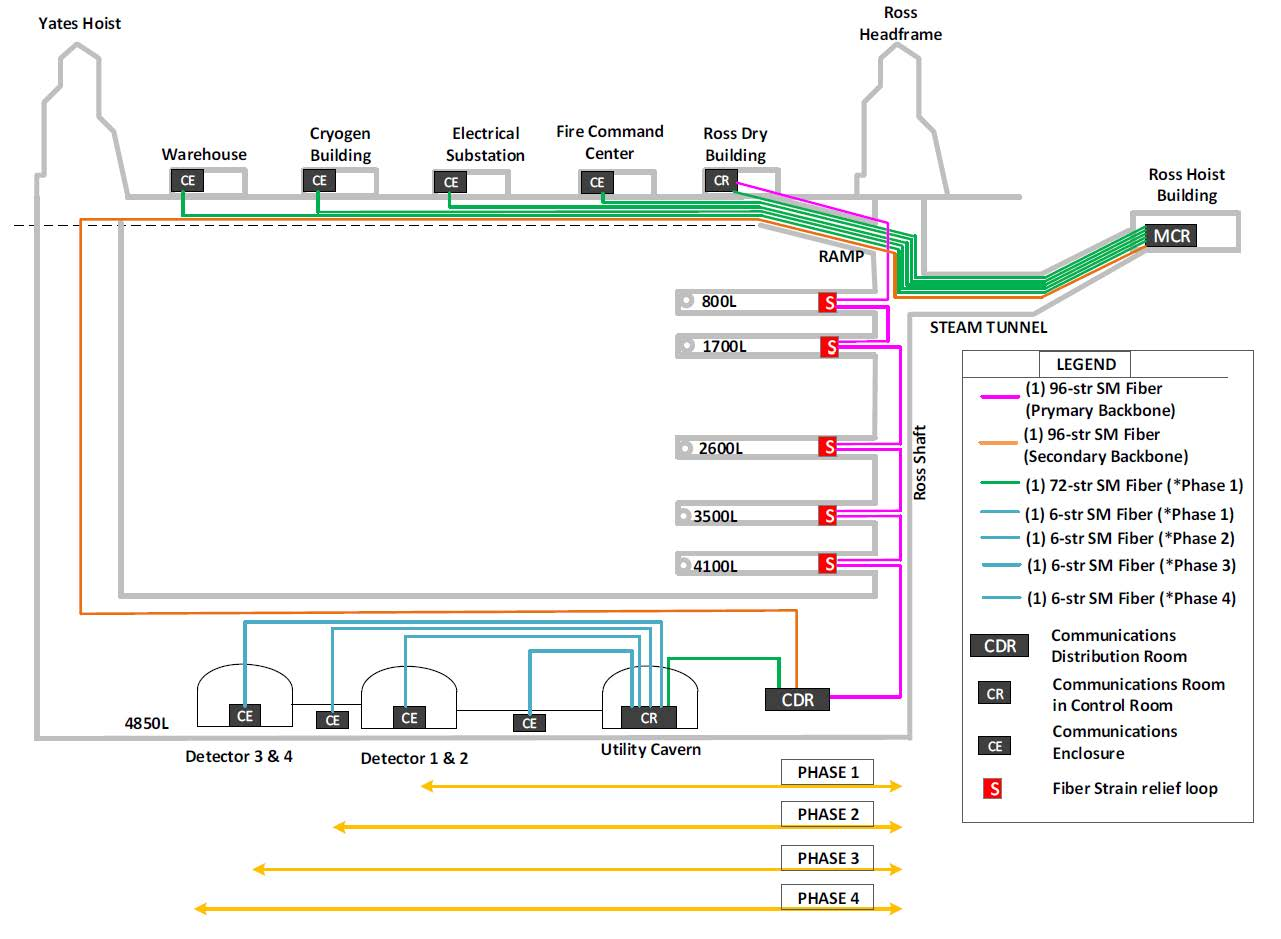
\includegraphics[width=1.0\textwidth]{fiber-distrib}
\end{cdrfigure}

Voice communications are provided via two-way radios and phones distributed throughout the underground spaces (in every room as well as every 500 ft in drifts). Two-way radios and cellular phones utilize a leaky feeder system to ensure communications over long distance without line of site. These leaky feeders are cables that act as antennas installed the length of all drifts and shafts. The leaky feeder is planned as a scope option.  Standard phones utilize Voice over Internet Protocol (VoIP) to provide communication though the fiber optic data backbone.

The data system is designed to provide 10-Gigabit Ethernet in the backbone and 1-Gigabit Ethernet to connected systems (computers). This system is intentionally left at a lesser level of design due to the continuous progression and advancement of technology that will almost certainly result in more advanced technologies than are currently available being utilized at the time of construction.

%%%%%%%%%%%%%%%%%%%%%%%%%%%%%%%%%%%%%%%%%%%%%%%%%%%%%%%%%%%%%%%%%%%
\section{Excavated Material Management}
\label{sec:fscf-und-waste-rock}

Prior to the commencement of any excavation activities, it will be necessary to establish an excavated-material management system and repository \fixme{Josh says: Need to determine whether this terminology is acceptable from Pepin}. The capacity of this system will be equivalent to what was in place during mining operations. 
There are a number of components to the management system, including refurbishing the Ross Shaft hoisting system and % the Ross Shaft 
crushers, and constructing a new conveying system.  As of this report, two options have been identified for final repositories of the material.  

The former Gilt Edge mine is located approximately seven miles from the SURF property and would require truck haulage as a component of the transportation system.  In this option, a new conveyor is provided to transport rock downhill to Kirk Road, as seen in Figure~\ref{fig:waste-rock-sys}. This is considered the reference design as of the date of this report.

\begin{cdrfigure}[Waste rock handling system route]{waste-rock-sys}{Waste-rock Handling System route (SRK, Courtesy SURF)}
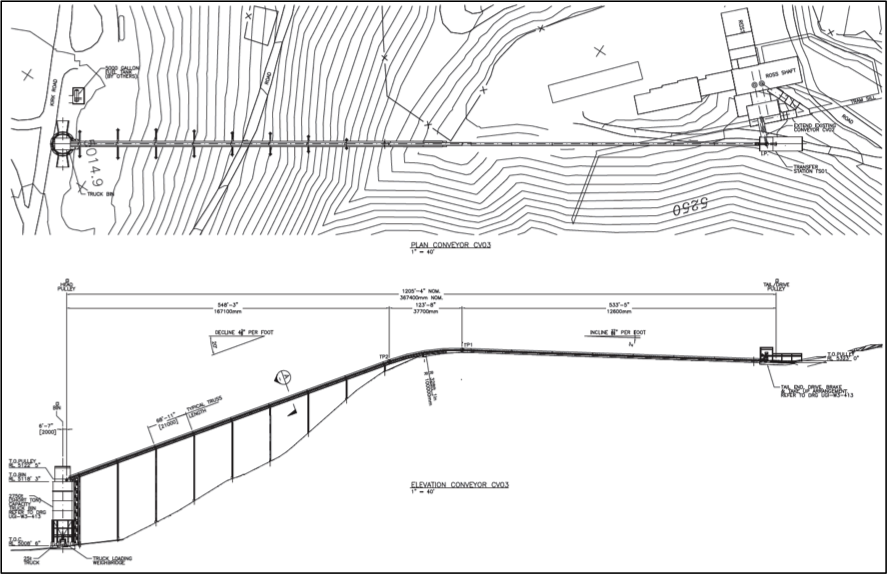
\includegraphics[width=0.8\textwidth]{waste-rock-sys}
\end{cdrfigure}

The alternative repository is the Homestake Open cut, located less than 1 mile from the SURF property.  In this option it is possible %A conveying system is possible in this option that would 
to transport material directly to the final location, avoiding the need for over-the road transportation.  The conveying system would be designed to follow a route formerly used to transport material from the open cut to the former Homestake mills. 

A final decision on which repository to use will be made prior to the CD-3a approval.  Both options have been evaluated in detail and are not significantly different in cost or installation schedule.  %The reference location as of this report is the Gilt Edge mine.

The systems utilize experience and equipment from the former Homestake Mining Company, % legacy, 
where rock was removed to the surface using skips in both the Yates and Ross Shafts. At the headframe of each shaft, the material was crushed to a nominal $3/4$~in, passed through ore bins, and was transported via underground rail to the mill system. All systems from the underground to the crushers will be rehabilitated from the original systems, though the material may not be required to be crushed as finely as it was during the mining period, and therefore some components of the system may not be re-used.




